% !TeX program = xelatex
\documentclass[a4paper,10pt]{article}

% ============================================================================
% កញ្ចប់បណ្ណាល័យ (Packages) – អនុវិទ្យាល័យព្រះក្រសាំង (គ្មាន LCD / សន្លឹកកិច្ចការជាគោល)
% ============================================================================
\usepackage[a4paper, left=0.95cm, right=0.95cm, top=0.85cm, bottom=0.92cm, footskip=0.52cm]{geometry}
\usepackage{amsmath}
\usepackage{unicode-math}
\usepackage{fontspec}
\usepackage{array, longtable, multirow, colortbl}
\usepackage[table]{xcolor}
\usepackage{enumitem}
\usepackage{pifont}
\usepackage{fancyhdr}
\usepackage{tikz}
\usetikzlibrary{calc, arrows.meta, decorations.pathreplacing, patterns, positioning, babel}

\makeatletter
\let\@expl@@@mark@update@singlecol@structures@@\relax
\makeatother

% ============================================================================
% ការកំណត់ពុម្ពអក្សរ (Cross-Platform Windows + Linux Cloud fonts/)
% ============================================================================
\providecommand{\NGSFindFonts}{%
  \IfFileExists{C:/Windows/Fonts/cambria.ttc}{%
    \def\NGSSysPath{C:/Windows/Fonts/}%
    \def\NGSUserPath{C:/Users/KIT/AppData/Local/Microsoft/Windows/Fonts/}%
  }{%
    \IfFileExists{./fonts/KhmerOSsiemreap.ttf}{\def\NGSSysPath{./fonts/}\def\NGSUserPath{./fonts/}}{%
    \IfFileExists{../fonts/KhmerOSsiemreap.ttf}{\def\NGSSysPath{../fonts/}\def\NGSUserPath{../fonts/}}{%
    \IfFileExists{../../fonts/KhmerOSsiemreap.ttf}{\def\NGSSysPath{../../fonts/}\def\NGSUserPath{../../fonts/}}{%
    \IfFileExists{../../../fonts/KhmerOSsiemreap.ttf}{\def\NGSSysPath{../../../fonts/}\def\NGSUserPath{../../../fonts/}}{%
    \IfFileExists{../../../../fonts/KhmerOSsiemreap.ttf}{\def\NGSSysPath{../../../../fonts/}\def\NGSUserPath{../../../../fonts/}}{%
    \IfFileExists{../../../../../fonts/KhmerOSsiemreap.ttf}{\def\NGSSysPath{../../../../../fonts/}\def\NGSUserPath{../../../../../fonts/}}{%
    \IfFileExists{../../../../../../fonts/KhmerOSsiemreap.ttf}{\def\NGSSysPath{../../../../../../fonts/}\def\NGSUserPath{../../../../../../fonts/}}{%
      \def\NGSSysPath{../../../../../../../fonts/}\def\NGSSysPath{../../../../../../../fonts/}%
    }}}}}}}%
  }%
}
\NGSFindFonts

\setmathfont[
  Path={\NGSSysPath},
  FontIndex=1,
  Scale=1.02
]{cambria.ttc}

\defaultfontfeatures{Ligatures=TeX}

\setmainfont[
  Path={\NGSUserPath},
  Extension=.ttf,
  Script=Khmer,
  BoldFont={KhmerOSsiemreap},
  BoldFeatures={FakeBold=1.8},
  ItalicFont={KhmerOSsiemreap},
  ItalicFeatures={FakeSlant=0.25},
  BoldItalicFont={KhmerOSsiemreap},
  BoldItalicFeatures={FakeBold=1.8, FakeSlant=0.25}
]{KhmerOSsiemreap}

\newfontfamily\muol[
  Path={\NGSUserPath},
  Extension=.ttf,
  Script=Khmer
]{KhmerOSmuollight}

\newfontfamily\TimesEn[
  Path={\NGSSysPath},
  Extension=.ttf,
  Scale=1.00,
  BoldFont={timesbd},
  ItalicFont={timesi},
  BoldItalicFont={timesbi}
]{times}

\newfontfamily\NagaBold[
  Path={\NGSUserPath},
  Extension=.ttf
]{AKbalthom Naga Bold}

\newfontfamily\CalibriFont[
  Path={\NGSSysPath},
  Extension=.ttf
]{calibri}

\newfontfamily\Tacteing[
  Path={\NGSUserPath}
]{TACTENG.TTF}

\newfontfamily\CourierBullet[
  Path={\NGSSysPath},
  Extension=.ttf
]{cour}
\newcommand{\wcirc}{{\CourierBullet\fontsize{9.5pt}{11pt}\selectfont o}}

\XeTeXlinebreaklocale "km"
\XeTeXlinebreakskip = 0pt plus 1pt minus 0.1pt

% ============================================================================
% ការកំណត់ពណ៌ និងទម្រង់ទំព័រ (Colors & Page Style)
% ============================================================================
\definecolor{stepgray}{HTML}{D9D9D9}
\definecolor{headgray}{HTML}{F2F2F2}
\definecolor{boxgray}{HTML}{D9D9D9}
\definecolor{darkred}{HTML}{C00000}
\definecolor{red5e}{HTML}{FF0000}

\pagestyle{fancy}
\fancyhf{}
\renewcommand{\headrulewidth}{0pt}
\fancyfoot[R]{\CalibriFont\fontsize{11pt}{13pt}\selectfont\thepage}

\setlength{\parindent}{0pt}
\setlength{\parskip}{0pt}
\setlength{\tabcolsep}{3.8pt}

\newcolumntype{L}[1]{>{\raggedright\arraybackslash}p{#1}}

% ============================================================================
% ម៉ាក្រូជំនួយ (Helper Macros)
% ============================================================================
\newcommand{\en}[1]{{\TimesEn #1}}
\newcommand{\enbf}[1]{{\TimesEn\textbf{#1}}}
\newcommand{\unit}[1]{\,\text{\en{#1}}}
\newcommand{\riel}{\,\text{៛}}
\newcommand{\usd}{\,\text{\en{\$}}}
\newcommand{\fiveE}[1]{{\NagaBold\fontsize{9.5pt}{13pt}\selectfont\textcolor{red5e}{#1}}}
\newcommand{\timenote}[1]{\textcolor{darkred}{\textit{#1}}}
\newcommand{\redsub}[1]{\textcolor{darkred}{#1}}
\newcommand{\graybox}[1]{\colorbox{boxgray}{\strut\hspace{2pt}#1\hspace{2pt}}}
\newcommand{\ditem}{\tikz[baseline=-0.5ex]\fill (0,0.42ex) -- (0.42ex,0) -- (0,-0.42ex) -- (-0.42ex,0) -- cycle;\hspace{0.3em}}
\newcommand{\cnum}[1]{{\fontsize{10.5pt}{12pt}\selectfont\ding{\numexpr181+#1\relax}}\hspace{0.15em}}
\newcommand{\cfig}[1]{\par\vspace{3pt}{\centering #1\par}\vspace{3pt}}
\newcommand{\stepheader}[1]{\multicolumn{3}{|c|}{\cellcolor{stepgray}\muol #1} \\* \noalign{\hrule height 0.4pt}}
\newcommand{\fboxb}[1]{\begingroup\setlength{\fboxsep}{1.5pt}\fbox{#1}\endgroup}
\newcommand{\khmflourish}{{\Tacteing\fontsize{36pt}{14pt}\selectfont\raisebox{-5pt}{3}}}

% ============================================================================
% ម៉ាក្រូគូសរូប TikZ ស-ខ្មៅ ១០០% (x=1cm, y=1cm, font=\scriptsize, width=7.55cm)
% ============================================================================

% ១. E1 Engage: បេសកកម្មដំឡើងថ្លៃ 20% រួចបញ្ចុះតម្លៃ 20%
\newcommand{\figEngagePCTThreeTwoThree}{%
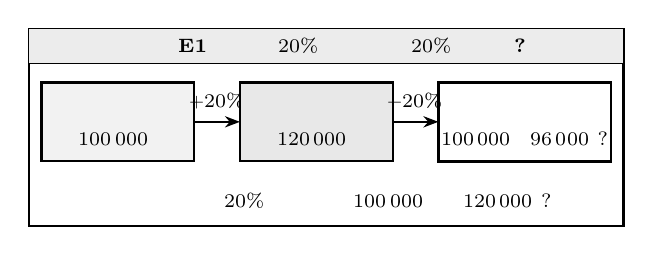
\begin{tikzpicture}[x=1cm, y=1cm, every node/.style={font=\scriptsize, text=black}]
  \draw[black, line width=0.9pt] (0,0) rectangle (7.55,2.50);
  \fill[gray!15] (0,2.06) rectangle (7.55,2.50);
  \draw[black, line width=0.6pt] (0,2.06) -- (7.55,2.06);
  \node at (3.775,2.28) {\textbf{បេសកកម្ម \en{E1}៖ ដំឡើងថ្លៃ $20\%$ រួចបញ្ចុះតម្លៃ $20\%$ ស្មើដើមឬទេ?}};

  \draw[black, line width=0.8pt, fill=gray!10] (0.16,0.82) rectangle (2.10,1.82);
  \node at (1.13,1.54) {\textbf{តម្លៃដើម}};
  \node at (1.13,1.10) {$100\,000\riel$};

  \draw[-{Stealth[length=1.9mm]}, line width=0.85pt] (2.10,1.32) -- (2.68,1.32) node[midway, above=1pt] {$+20\%$};

  \draw[black, line width=0.8pt, fill=gray!18] (2.68,0.82) rectangle (4.62,1.82);
  \node at (3.65,1.54) {\textbf{ក្រោយដំឡើង}};
  \node at (3.65,1.10) {$120\,000\riel$};

  \draw[-{Stealth[length=1.9mm]}, line width=0.85pt] (4.62,1.32) -- (5.20,1.32) node[midway, above=1pt] {$-20\%$};

  \draw[black, line width=0.95pt] (5.20,0.82) rectangle (7.39,1.82);
  \node at (6.295,1.54) {\textbf{តម្លៃលក់ចុងក្រោយ}};
  \node at (6.295,1.10) {$100\,000$ ឬ $96\,000\riel$?};

  \node at (3.775,0.32) {\textbf{សំណួរគន្លឹះ៖} តើបញ្ចុះ $20\%$ លើកទី ២ គិតលើ $100\,000\riel$ ឬលើ $120\,000\riel$?};
\end{tikzpicture}}

% ២. E2 Act 1: បន្ទះការបញ្ចុះតម្លៃ (កាបូបដៃ 32 000 -> 25 600 និងសម្លៀកបំពាក់បញ្ចុះ 30% ទំ.៣៣-៣៤)
\newcommand{\figDiscountBarPCTThreeTwoThree}{%
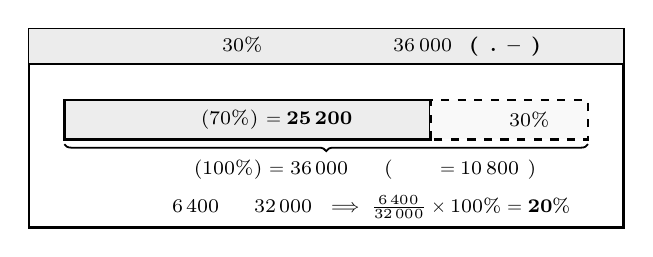
\begin{tikzpicture}[x=1cm, y=1cm, every node/.style={font=\scriptsize, text=black}]
  \draw[black, line width=0.9pt] (0,0) rectangle (7.55,2.52);
  \fill[gray!15] (0,2.08) rectangle (7.55,2.52);
  \draw[black, line width=0.6pt] (0,2.08) -- (7.55,2.08);
  \node at (3.775,2.30) {\textbf{បន្ទះការបញ្ចុះតម្លៃ $30\%$ លើសម្លៀកបំពាក់ថ្លៃដើម $36\,000\riel$ (ទំ.៣៣--៣៤)}};

  % Bar from 0.45 to 7.10 (length 6.65 cm; 70% = 4.655 cm)
  \draw[black, line width=0.85pt, fill=gray!14] (0.45,1.12) rectangle (5.10,1.62);
  \node at (2.775,1.37) {ថ្លៃលក់ថ្មី ($70\%$) $= \mathbf{25\,200\riel}$};
  \draw[black, line width=0.85pt, dashed, fill=gray!5] (5.10,1.12) rectangle (7.10,1.62);
  \node at (6.10,1.37) {បញ្ចុះ $30\%$};

  \draw[decorate, decoration={brace, mirror, amplitude=2.5pt}, line width=0.65pt] (0.45,1.06) -- (7.10,1.06);
  \node at (3.775,0.74) {ថ្លៃលក់ខាងដើម ($100\%$) $= 36\,000\riel$ \quad (\text{បញ្ចុះ } $= 10\,800\riel$)};
  \node at (3.775,0.26) {កាបូបដៃ៖ បញ្ចុះ $6\,400\riel$ លើ $32\,000\riel \implies \frac{6\,400}{32\,000}\times 100\% = \mathbf{20\%}$};
\end{tikzpicture}}

% ៣. E3 Explain: ដ្យាក្រាមព្រួញមេគុណទៅ-មក (Forward vs Reverse Multiplier Arrow)
\newcommand{\figMultiplierArrowPCTThreeTwoThree}{%
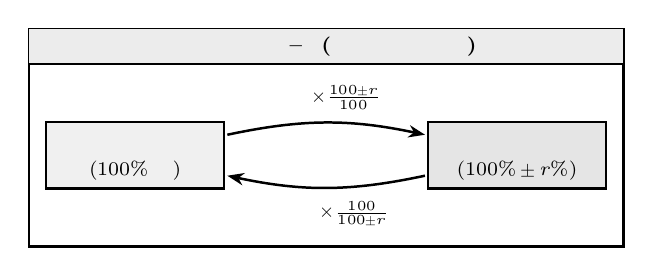
\begin{tikzpicture}[x=1cm, y=1cm, every node/.style={font=\scriptsize, text=black}]
  \draw[black, line width=0.9pt] (0,0) rectangle (7.55,2.76);
  \fill[gray!15] (0,2.32) rectangle (7.55,2.76);
  \draw[black, line width=0.6pt] (0,2.32) -- (7.55,2.32);
  \node at (3.775,2.54) {\textbf{ដ្យាក្រាមព្រួញមេគុណទៅ–មក (បំបែកអន្ទាក់ភាគរយបញ្ច្រាស)}};

  \draw[black, line width=0.9pt, fill=gray!12] (0.22,0.74) rectangle (2.48,1.58);
  \node at (1.35,1.32) {\textbf{តម្លៃដើម}};
  \node at (1.35,0.96) {($100\%$ គោល)};

  \draw[black, line width=0.9pt, fill=gray!20] (5.07,0.74) rectangle (7.33,1.58);
  \node at (6.20,1.32) {\textbf{តម្លៃថ្មី}};
  \node at (6.20,0.96) {($100\% \pm r\%$)};

  % Forward arrow (top)
  \draw[-{Stealth[length=2.1mm]}, line width=0.9pt] (2.52,1.42) to[bend left=12] node[above=1pt] {ទៅមុខ៖ $\times \tfrac{100\pm r}{100}$} (5.03,1.42);

  % Reverse arrow (bottom)
  \draw[-{Stealth[length=2.1mm]}, line width=0.9pt] (5.03,0.90) to[bend left=12] node[below=1pt] {បញ្ច្រាស៖ $\times \tfrac{100}{100\pm r}$} (2.52,0.90);
\end{tikzpicture}}

% ៤. E4 Elaborate: ប្រាក់ខែដំឡើង 8% (លោកប៊ុនថា ទៅមុខ vs លោកស្រីចាន់ធី បញ្ច្រាស ទំ.៣៤-៣៥)
\newcommand{\figElaborateSalaryPCTThreeTwoThree}{%
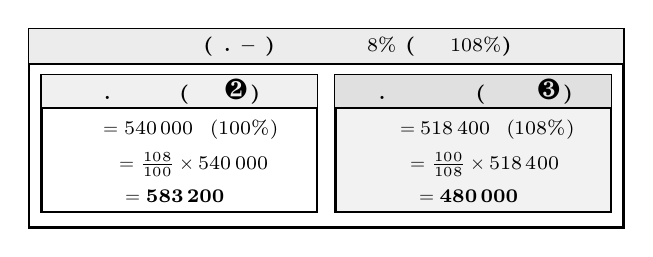
\begin{tikzpicture}[x=1cm, y=1cm, every node/.style={font=\scriptsize, text=black}]
  \draw[black, line width=0.9pt] (0,0) rectangle (7.55,2.52);
  \fill[gray!15] (0,2.08) rectangle (7.55,2.52);
  \draw[black, line width=0.6pt] (0,2.08) -- (7.55,2.08);
  \node at (3.775,2.30) {\textbf{លំហាត់គំរូ (ទំ.៣៤--៣៥)៖ ដំឡើងប្រាក់ខែ $8\%$ ($\text{មេគុណ } 108\%$)}};

  % Left: Forward
  \draw[black, line width=0.8pt] (0.16,0.20) rectangle (3.66,1.94);
  \fill[gray!12] (0.16,1.52) rectangle (3.66,1.94);
  \draw[black, line width=0.55pt] (0.16,1.52) -- (3.66,1.52);
  \node at (1.91,1.73) {\textbf{ក. លោកប៊ុនថា (ទៅមុខ \cnum{2})}};
  \node at (1.91,1.24) {ដើម $= 540\,000\riel$ ($100\%$)};
  \node at (1.91,0.80) {ថ្មី $= \tfrac{108}{100}\times 540\,000$};
  \node at (1.91,0.40) {$= \mathbf{583\,200\riel}$};

  % Right: Reverse
  \draw[black, line width=0.95pt, fill=gray!10] (3.89,0.20) rectangle (7.39,1.94);
  \fill[gray!24] (3.89,1.52) rectangle (7.39,1.94);
  \draw[black, line width=0.6pt] (3.89,1.52) -- (7.39,1.52);
  \node at (5.64,1.73) {\textbf{ខ. លោកស្រីចាន់ធី (បញ្ច្រាស \cnum{3})}};
  \node at (5.64,1.24) {ថ្មី $= 518\,400\riel$ ($108\%$)};
  \node at (5.64,0.80) {ដើម $= \tfrac{100}{108}\times 518\,400$};
  \node at (5.64,0.40) {$= \mathbf{480\,000\riel}$};
\end{tikzpicture}}

% ៥. E5 Evaluate: ជម្រើសវិនិច្ឆ័យ A-D (អាវបញ្ចុះតម្លៃ 20% នៅសល់ 40 000៛ រកថ្លៃដើម)
\newcommand{\figExitPCTThreeTwoThree}{%
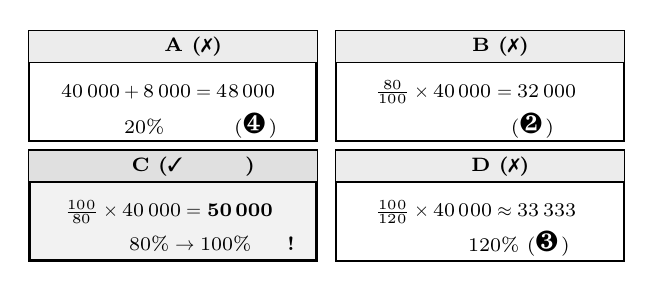
\begin{tikzpicture}[x=1cm, y=1cm, every node/.style={font=\scriptsize, text=black}]
  % A
  \draw[black, line width=0.8pt] (0,1.52) rectangle (3.65,2.92);
  \fill[gray!15] (0,2.52) rectangle (3.65,2.92);
  \draw[black, line width=0.55pt] (0,2.52) -- (3.65,2.52);
  \node at (1.825,2.72) {\textbf{ជម្រើស \en{A} (\ding{55})}};
  \node at (1.825,2.14) {$40\,000 + 8\,000 = 48\,000\riel$};
  \node at (1.825,1.72) {អន្ទាក់យក $20\%$ លើថ្លៃថ្មី (\cnum{4})};

  % B
  \draw[black, line width=0.8pt] (3.90,1.52) rectangle (7.55,2.92);
  \fill[gray!15] (3.90,2.52) rectangle (7.55,2.92);
  \draw[black, line width=0.55pt] (3.90,2.52) -- (7.55,2.52);
  \node at (5.725,2.72) {\textbf{ជម្រើស \en{B} (\ding{55})}};
  \node at (5.725,2.14) {$\tfrac{80}{100}\times 40\,000 = 32\,000\riel$};
  \node at (5.725,1.72) {ច្រឡំបញ្ចុះម្ដងទៀត (\cnum{2})};

  % C (Correct)
  \draw[black, line width=1.1pt, fill=gray!10] (0,0) rectangle (3.65,1.40);
  \fill[gray!24] (0,1.00) rectangle (3.65,1.40);
  \draw[black, line width=0.6pt] (0,1.00) -- (3.65,1.00);
  \node at (1.825,1.20) {\textbf{ជម្រើស \en{C} (\ding{51} ត្រឹមត្រូវ)}};
  \node at (1.825,0.62) {$\tfrac{100}{80}\times 40\,000 = \mathbf{50\,000\riel}$};
  \node at (1.825,0.22) {\textbf{ព្រួញបញ្ច្រាស $80\% \to 100\%$ ត្រូវ!}};

  % D
  \draw[black, line width=0.8pt] (3.90,0) rectangle (7.55,1.40);
  \fill[gray!15] (3.90,1.00) rectangle (7.55,1.40);
  \draw[black, line width=0.55pt] (3.90,1.00) -- (7.55,1.00);
  \node at (5.725,1.20) {\textbf{ជម្រើស \en{D} (\ding{55})}};
  \node at (5.725,0.62) {$\tfrac{100}{120}\times 40\,000 \approx 33\,333\riel$};
  \node at (5.725,0.22) {ច្រឡំសញ្ញាបូក $120\%$ (\cnum{3})};
\end{tikzpicture}}

% ============================================================================
% ចាប់ផ្ដើមឯកសារ (Document Body)
% ============================================================================
\begin{document}
\fontsize{10pt}{15.2pt}\selectfont

% -------------------- ក្បាលកិច្ចតែងការ (Header) --------------------
\begin{center}
  {\muol\fontsize{11pt}{16pt}\selectfont ព្រះរាជាណាចក្រកម្ពុជា}\\[2pt]
  {\muol\fontsize{10pt}{15pt}\selectfont ជាតិ សាសនា ព្រះមហាក្សត្រ}\\[1pt]
  \khmflourish
\end{center}

\vspace{-24pt}
{\muol\fontsize{9.5pt}{12.5pt}\selectfont
មន្ទីរអប់រំ យុវជន និងកីឡា ខេត្តកំពង់ធំ\\
ការិយាល័យអប់រំ យុវជន និងកីឡា ស្រុកកំពង់ស្វាយ\\
អនុវិទ្យាល័យព្រះក្រសាំង}

\vspace{1pt}
\begin{center}
  {\muol\fontsize{10pt}{14pt}\selectfont កិច្ចតែងការបង្រៀន}
\end{center}
\vspace{0pt}

% -------------------- ព័ត៌មានទូទៅ (Metadata) --------------------
{\renewcommand{\arraystretch}{0.98}
\hspace*{3.1cm}%
\begin{tabular}{@{}l l L{11.0cm}@{}}
  - \hspace{0.35cm} មុខវិជ្ជា & : & គណិតវិទ្យា ថ្នាក់ទី៨ (ពីជគណិត) \\
  - \hspace{0.35cm} ចំណងជើងមេរៀន & : & មេរៀនទី៣៖ ទំហំសមាមាត្រនិងភាគរយ \\
  - \hspace{0.35cm} ចំណងជើងរង & : & ២.៣–២.៤. ការបញ្ចុះតម្លៃ និងបម្រែបម្រួលភាគរយ (ទំ.៣៣–៣៥, ៤២) \\
  - \hspace{0.35cm} រយៈពេល & : & ១ ម៉ោងសិក្សា (៥០ នាទី) \\
  - \hspace{0.35cm} បង្រៀនដោយ & : & ហុក ប៊ុនថែន \\
  - \hspace{0.35cm} កាលបរិច្ឆេទ & : & ថ្ងៃចន្ទ ទី២៣ ខែវិច្ឆិកា ឆ្នាំ២០២៦ \\
\end{tabular}

\vspace{2pt}

% -------------------- I. វត្ថុបំណង --------------------
\textbf{I.} {\muol វត្ថុបំណង}\\[1pt]
\hspace*{0.55cm}%
\begin{tabular}{@{}l l L{14.2cm}@{}}
  \wcirc \hspace{0.25cm} វិជ្ជាសម្បទា & : & សិស្សប្រាប់និយមន័យនិងរូបមន្តភាគរយនៃការបញ្ចុះតម្លៃធៀបនឹងថ្លៃលក់ខាងដើម និងប្រាប់ទំនាក់ទំនងផលធៀបនៃបម្រែបម្រួលភាគរយ ($\frac{\text{តម្លៃថ្មី}}{\text{តម្លៃដើម}} = \frac{100 \pm r}{100}$) បានត្រឹមត្រូវ ។ \\
  \wcirc \hspace{0.25cm} បំណិនសម្បទា & : & សិស្សគណនាភាគរយការបញ្ចុះតម្លៃ ថ្លៃលក់ថ្មី តម្លៃបន្ទាប់ពីកើនឬថយភាគរយ និងរកតម្លៃដើមបញ្ច្រាស ($\times\frac{100}{100\pm r}$) លើសន្លឹកកិច្ចការតាមលំហាត់ជីវភាពពិត (ទំ.៣៣–៣៥) បានត្រឹមត្រូវ ។ \\
  \wcirc \hspace{0.25cm} ចរិយាសម្បទា & : & សិស្សមានភាពវៃឆ្លាតក្នុងការពិនិត្យស្លាកបញ្ចុះតម្លៃទំនិញលើទីផ្សារ ប្រុងប្រយ័ត្នចំពោះតម្លៃគោល $100\%$ មុនគណនា និងចេះសន្សំសំចៃថវិកាគ្រួសារ ។ \\
\end{tabular}

\vspace{2pt}

% -------------------- II. សម្ភារៈឧបទេស --------------------
\textbf{II.} {\muol សម្ភារៈឧបទេស}\\[1pt]
\hspace*{0.55cm}$\bullet$ \hspace{0.35cm} សៀវភៅសិក្សាគោលថ្នាក់ទី៨ (ទំ.៣៣–៣៥, ៤២) ក្ដារខៀន ដីស/ហ្វឺត បន្ទាត់ត្រង់ និង\textbf{សន្លឹកកិច្ចការសិស្សបំពេញចន្លោះ ស-ខ្មៅ} (\en{Printable\_Materials\_PCT323} ទំព័រ ១–២ សម្រាប់សិស្ស និងទំព័រ ៣ ប្លង់ក្ដារខៀន/ចម្លើយគ្រូ — គ្មានប្រើ \en{LCD})

\vspace{2pt}

% -------------------- III. វិធីសាស្រ្តបង្រៀន --------------------
\textbf{III.} {\muol វិធីសាស្រ្តបង្រៀន}\\[1pt]
\hspace*{0.45cm}%
\begin{tabular}{@{}l l L{14.85cm}@{}}
  $\bullet$ \hspace{0.25cm} គោលវិធី & : & សិស្សមជ្ឈមណ្ឌល (សន្លឹកកិច្ចការបំពេញចន្លោះជាគោល + ការពិភាក្សាជាក្រុមតូច ៣ នាក់) \\
  $\bullet$ \hspace{0.25cm} យុទ្ធវិធីបង្រៀន & : & គំរូស្ថាបនានិយម \en{5Es} រួមបញ្ចូល \textbf{ដ្យាក្រាមព្រួញមេគុណទៅ–មក (\en{Forward--Reverse Multiplier Arrow})} និង \textbf{ការវិភាគករណីផ្ទុយភាគរយបញ្ច្រាស} \\
\end{tabular}
}

\vspace{2pt}

% -------------------- IV. ដំណើរការបង្រៀន --------------------
\textbf{IV.} {\muol ដំណើរការបង្រៀន}

\vspace{1pt}
{\renewcommand{\arraystretch}{1.12}
\begin{longtable}{|L{5.50cm}|L{7.90cm}|L{4.80cm}|}
\hline
\multicolumn{1}{|c|}{\cellcolor{headgray}\muol សកម្មភាពគ្រូ} &
\multicolumn{1}{c|}{\cellcolor{headgray}\muol ខ្លឹមសារមេរៀន} &
\multicolumn{1}{c|}{\cellcolor{headgray}\muol សកម្មភាពសិស្ស} \\
\endhead
\hline
\endfoot

% ==================== ជំហានទី១ (2min) ====================
\stepheader{ជំហានទី១ \enbf{(}រដ្ឋបាលថ្នាក់\enbf{)}}
$\bullet$ ពិនិត្យវត្តមាន អនាម័យ និងសណ្ដាប់ធ្នាប់ថ្នាក់រៀន \par
$\bullet$ រៀបចំក្រុមតូច ៣ នាក់តាមតុ និងចែក\textbf{សន្លឹកកិច្ចការសិស្ស (\en{PCT323} ទំព័រ ១–២)}
&
$\bullet$ រដ្ឋបាលថ្នាក់ អនាម័យ និងវិន័យសិក្សា \par
$\bullet$ ចែកសន្លឹកកិច្ចការម្នាក់ ១ សន្លឹក សម្រាប់បំពេញតាមដំណាក់កាល \en{E1--E5}
&
$\circ$ ប្រធានថ្នាក់រាយការណ៍វត្តមានសិស្ស \par
$\circ$ ទទួលសន្លឹកកិច្ចការ សរសេរឈ្មោះ និងអង្គុយតាមក្រុម ៣ នាក់ \\
\hline

% ==================== ជំហានទី២ (9min: កំណែ <=3m + រំលឹក 3m + E1 3m) ====================
\stepheader{ជំហានទី២ \enbf{(}កិច្ចការផ្ទះ \enbf{+} ទំនាក់ទំនងមេរៀនថ្មី\enbf{)}}
\ditem \textbf{កំណែកិច្ចការផ្ទះ ($\le\text{\enbf{3\,min}}$)} \par
$\bullet$ ហៅសិស្ស ២ នាក់ឡើងកែលំហាត់ ទំ.៤១–៤២ លេខ ១៤(ក) និងលេខ ១៥ លើក្ដារខៀន
&
{\centering\redsub{កំណែកិច្ចការផ្ទះមេរៀនមុន (ទំ.៤១–៤២ \#14 ក និង \#15)}\par}
$\bullet$ \textbf{\#14 ក៖} $72\% - 28\% = 44\%$ ត្រូវនឹង $1\,980$ ក្បាល $\implies$ សរុប $\mathbf{4\,500}$ ក្បាល (ប្រលោមលោក $\mathbf{1\,260}$, មិនមែនប្រលោមលោក $\mathbf{3\,240}$ ក្បាល) \par
$\bullet$ \textbf{\#15៖} សល់ពីចំណាយ $200\,000\usd$; លោកសុងបាន $32\,000\usd + 48\,000\usd = \mathbf{80\,000\usd}$, លោកចេន $\mathbf{54\,000\usd}$, លោកស្រីភី $\mathbf{66\,000\usd}$
&
$\circ$ ផ្ទៀងចម្លើយ និងកែតម្រូវចូលសៀវភៅកិច្ចការផ្ទះ \\[3pt]

\ditem \textbf{រំលឹកមេរៀនទាក់ទង (\enbf{3min})} \par
$\bullet$ សួររំលឹក៖ «បើពូសុខលក់ម៉ូតូខាត $22\%$ តើថ្លៃលក់ស្មើប៉ុន្មានភាគរយនៃថ្លៃដើម $100\%$?»
&
{\centering\redsub{រំលឹកទំនាក់ទំនងភាគរយនៅសល់ (២.២)}\par}
$\bullet$ ថ្លៃដើមស្មើ $100\%$៖ បើលក់ខាត $22\%$ នោះថ្លៃលក់នៅសល់ $100\% - 22\% = \mathbf{78\%}$ នៃថ្លៃដើម ។
&
$\circ$ ឆ្លើយ៖ «នៅសល់ $100\% - 22\% = 78\%$ នៃថ្លៃដើម!» \\[3pt]

\fiveE{E1 - Engage (3min)} \timenote{(កុំទាន់ផ្ដល់ចម្លើយ)} \par
\ditem \textbf{បេសកកម្មស្លាកបញ្ចុះតម្លៃ (សន្លឹកកិច្ចការ \en{E1})} \par
$\bullet$ ឱ្យសិស្សអានប្រអប់ \en{E1} ហើយគូសជ្រើសរើសរវាង \textbf{$100\,000\riel$} និង \textbf{$96\,000\riel$}
&
\redsub{បេសកកម្ម \en{E1}៖ ដំឡើង $20\%$ រួចបញ្ចុះតម្លៃ $20\%$} \par
ហាងមួយដំឡើងថ្លៃអាវពី $100\,000\riel$ ឡើង $20\%$ បាន $120\,000\riel$ ។ សប្ដាហ៍ក្រោយហាងប្រកាសបញ្ចុះតម្លៃ $20\%$ លើថ្លៃថ្មីនោះ! \par
$\bullet$ តើតម្លៃលក់ចុងក្រោយត្រឡប់មក $100\,000\riel$ វិញ ឬស្មើ $96\,000\riel$?
&
$\circ$ ពិភាក្សាជាគូ និងគូស \ding{51} ក្នុងប្រអប់ \en{E1} លើសន្លឹកកិច្ចការ \\[3pt]

&
\cfig{\figEngagePCTThreeTwoThree}
& \\
\hline

% ==================== ជំហានទី៣ (17min: E2 11m + E3 6m) ====================
\stepheader{ជំហានទី៣ \enbf{(}ខ្លឹមសារមេរៀនថ្មី\enbf{)}}
\fiveE{E2 - Explore (11min)} \par
$\bullet$ សរសេរចំណងជើងរង \textbf{២.៣. ការបញ្ចុះតម្លៃ} និង \textbf{២.៤. បម្រែបម្រួលភាគរយ} \par
\ditem \textbf{សកម្មភាព ១៖ ការបញ្ចុះតម្លៃកាបូបដៃ និងសម្លៀកបំពាក់ (\enbf{5min}, សន្លឹកកិច្ចការ \en{E2-A})} \par
$\bullet$ ឱ្យសិស្សដោះស្រាយលំហាត់គំរូទំ.៣៣–៣៤ លើសន្លឹកកិច្ចការ \en{E2-A}
&
មេរៀនទី៣ \quad {\muol ទំហំសមាមាត្រនិងភាគរយ \enbf{(}ត\enbf{)}} \par
២.៣. ការបញ្ចុះតម្លៃ \par
$\bullet$ \textbf{លំហាត់គំរូ (ទំ.៣៣–៣៤)៖} \par
\hspace*{0.2cm}-- \textbf{ក. កាបូបដៃ៖} ដើម $32\,000\riel$, លក់ $25\,600\riel \implies$ បញ្ចុះ $6\,400\riel$ \par
\hspace*{0.5cm}$\implies \text{ភាគរយបញ្ចុះតម្លៃ} = \dfrac{6\,400}{32\,000}\times 100\% = \mathbf{20\%}$ \par
\hspace*{0.2cm}-- \textbf{ខ. សម្លៀកបំពាក់៖} ដើម $36\,000\riel$, បញ្ចុះ $30\%$ ($=10\,800\riel$) \par
\hspace*{0.5cm}$\implies \text{ថ្លៃលក់} = 36\,000 - 10\,800 = \mathbf{25\,200\riel}$ (ឬ $70\%\times 36\,000\riel$)
&
$\circ$ បំពេញការគណនាឃើញកាបូបបញ្ចុះ $20\%$ និងសម្លៀកបំពាក់លក់ថ្លៃ $25\,200\riel$ \\[3pt]

&
\cfig{\figDiscountBarPCTThreeTwoThree}
& \\[3pt]

\ditem \textbf{សកម្មភាព ២៖ មេគុណបម្រែបម្រួលភាគរយ (\enbf{6min}, សន្លឹកកិច្ចការ \en{E2-B})} \par
$\bullet$ ឱ្យសិស្សពិនិត្យឧទាហរណ៍ប្រាក់ខែកម្មករ $320\,000\riel$ កើន $15\%$ និងថយចុះ $5\%$ (សៀវភៅទំ.៣៤)
&
២.៤. បម្រែបម្រួលភាគរយ \par
$\bullet$ \textbf{ឧទាហរណ៍ (ទំ.៣៤ — ប្រាក់ខែដើម $320\,000\riel$)៖} \par
\hspace*{0.2cm}-- កើន $15\%$ ($\frac{\text{ថ្មី}}{\text{ដើម}} = \frac{115}{100}$)៖ $\text{ប្រាក់ខែថ្មី} = \dfrac{115}{100}\times 320\,000 = \mathbf{368\,000\riel}$ \par
\hspace*{0.2cm}-- ថយចុះ $5\%$ ($\frac{\text{ថ្មី}}{\text{ដើម}} = \frac{95}{100}$)៖ $\text{ប្រាក់ខែថ្មី} = \dfrac{95}{100}\times 320\,000 = \mathbf{304\,000\riel}$
&
$\circ$ គណនាតាមផលធៀប $\frac{115}{100}$ និង $\frac{95}{100}$ លើសន្លឹកកិច្ចការ \en{E2-B} \\[3pt]

% --- E3 Explain (6min) ---
\fiveE{E3 - Explain (6min)} \par
$\bullet$ ដឹកនាំសិស្សសង្ខេបរូបមន្ត\textbf{ការបញ្ចុះតម្លៃ ២.៣} លើក្ដារខៀន និងសន្លឹកកិច្ចការ \en{E3}
&
$\bullet$ \textbf{រូបមន្តការបញ្ចុះតម្លៃ (ទំ.៣៣)៖} \par
\hspace*{0.3cm}\graybox{$\text{ភាគរយការបញ្ចុះតម្លៃ} = \dfrac{\text{ការបញ្ចុះតម្លៃ}}{\text{ថ្លៃលក់ខាងដើម}}\times 100\%$}
&
$\circ$ បំពេញប្រអប់រូបមន្ត ២.៣ លើសន្លឹកកិច្ចការ \en{E3} \\[3pt]

$\bullet$ បន្តដឹកនាំសិស្សសង្ខេបប្រព័ន្ធ\textbf{ព្រួញមេគុណទៅ–មក ២.៤} (ទំ.៣៤–៣៥)
&
$\bullet$ \textbf{រូបមន្តបម្រែបម្រួលភាគរយ $r\%$ (ទំ.៣៤–៣៥)៖} \par
\hspace*{0.3cm}\graybox{$\text{តម្លៃថ្មី} = \dfrac{100 \pm r}{100}\times \text{តម្លៃដើម}$} \quad និងបញ្ច្រាស៖ \quad \graybox{$\text{តម្លៃដើម} = \dfrac{100}{100 \pm r}\times \text{តម្លៃថ្មី}$}
&
$\circ$ បំពេញប្រអប់រូបមន្តទៅមុខ និងបញ្ច្រាស ២.៤ លើសន្លឹកកិច្ចការ \en{E3} \\[3pt]

&
\cfig{\figMultiplierArrowPCTThreeTwoThree}
& \\[3pt]

$\bullet$ ភ្ជាប់\textbf{ធនាគារហេតុផល \cnum{1}--\cnum{4}} សម្រាប់ការពារអន្ទាក់ភាគរយបញ្ច្រាស
&
\textbf{ធនាគារហេតុផល (\en{Warrant Bank})៖} \par
\cnum{1} \textbf{ថ្លៃលក់ខាងដើម $= 100\%$៖} ភាគរយបញ្ចុះតម្លៃធៀបនឹងថ្លៃលក់ខាងដើមជានិច្ច \par
\cnum{2} \textbf{ព្រួញទៅមុខ (រកតម្លៃថ្មី)៖} គុណតម្លៃដើមនឹង $\frac{100+r}{100}$ (កើន) ឬ $\frac{100-r}{100}$ (បញ្ចុះ) \par
\cnum{3} \textbf{ព្រួញបញ្ច្រាស (រកតម្លៃដើម)៖} គុណតម្លៃថ្មីនឹងប្រភាគចម្រាស $\frac{100}{100\pm r}$ \par
\cnum{4} \textbf{បម្រាមដាច់ខាត៖} ហាមយក $r\%$ នៃតម្លៃថ្មីទៅបូក/ដកដើម្បីរកតម្លៃដើម!
&
$\circ$ ផ្ទៀងលេខកូដ \cnum{1}--\cnum{4} លើសន្លឹកកិច្ចការ \\
\hline

% ==================== ជំហានទី៤ (20min: E4 10m + E5 10m) ====================
\stepheader{ជំហានទី៤ \enbf{(}ពង្រីកចំណេះដឹង\enbf{)}}
\fiveE{E4 - Elaborate (10min)} \par
\ditem \textbf{លំហាត់គំរូ៖ ដំឡើងប្រាក់ខែ $8\%$ ទៅមុខ និងបញ្ច្រាស (ទំ.៣៤–៣៥)} \par
$\bullet$ ឱ្យសិស្សបំពេញ (ក) លោកប៊ុនថា និង (ខ) លោកស្រីចាន់ធី លើសន្លឹកកិច្ចការ \en{E4}
&
{\muol លំហាត់គំរូ} \textbf{(ទំ.៣៤–៣៥ — ក្រុមហ៊ុនអគ្គិសនីដំឡើងប្រាក់ខែ $8\%$)៖} \par
មេគុណបន្ទាប់ពីដំឡើង $8\%$ គឺ $100\% + 8\% = 108\% = \frac{108}{100}$ ៖ \par
$\bullet$ \textbf{ក. លោកប៊ុនថា (ស្គាល់ដើម $540\,000\riel$ — \cnum{2})៖} \par
\hspace*{0.3cm}$\text{ប្រាក់ខែថ្មី} = \dfrac{108}{100}\times 540\,000 = \graybox{$583\,200\riel$}$ \par
$\bullet$ \textbf{ខ. លោកស្រីចាន់ធី (ស្គាល់ថ្មី $518\,400\riel$ — \cnum{3})៖} \par
\hspace*{0.3cm}$\text{ប្រាក់ខែដើម} = \dfrac{100}{108}\times 518\,400 = \graybox{$480\,000\riel$}$
&
$\circ$ ញែកដាច់រវាងការគណនាទៅមុខ ($\frac{108}{100}$) និងបញ្ច្រាស ($\frac{100}{108}$) ឃើញ $583\,200\riel$ និង $480\,000\riel$ \\[3pt]

&
\cfig{\figElaborateSalaryPCTThreeTwoThree}
& \\[3pt]

$\bullet$ សួរសំណួរឆ្លុះបញ្ចាំង \textbf{\en{EIA Looking-Back} (1min)}
&
\textbf{\en{EIA Looking-Back}៖} «ក្នុងសំណួរ (ខ) បើសិស្សយក $518\,400 - 8\%(518\,400) = 476\,928\riel$ ហេតុអ្វីខុស?» ($\to$ ព្រោះ $8\%$ គឺដំឡើងលើប្រាក់ខែដើម $480\,000\riel$ មិនមែនលើប្រាក់ខែថ្មី $518\,400\riel$ ទេ តាម \cnum{4}! ផ្ទៀង៖ $480\,000 \times 1.08 = 518\,400\riel$ ត្រូវគ្នាគត់!)
&
$\circ$ ផ្ទៀងផ្ទាត់ទៅមុខ $480\,000\times 1.08 = 518\,400\riel$ \\[3pt]

% --- E5 Evaluate (10min) ---
\fiveE{E5 - Evaluate (10min)} \par
\ditem \textbf{ប្រតិបត្តិជាក្រុមតូច ៣ នាក់ (4min, សន្លឹកកិច្ចការ \en{E5})} \par
$\bullet$ ឱ្យសិស្សដោះស្រាយ \textbf{ប្រតិបត្តិទំ.៣៥ (ទោចក្រយានបញ្ចុះតម្លៃ $15\%$)}
&
{\muol លំហាត់ប្រតិបត្តិ} \textbf{(ទំ.៣៥ — កង់បញ្ចុះតម្លៃ $15\%$)៖} \par
$\bullet$ បញ្ចុះ $15\% \implies$ ថ្លៃថ្មីស្មើ $85\%$ នៃថ្លៃដើម (\cnum{3})៖ \par
\hspace*{0.3cm}$\text{ថ្លៃដើម} = \dfrac{100}{85}\times 846\,000 = 995\,294\dfrac{2}{17}\riel \approx \graybox{$995\,294.12\riel$}$
&
$\circ$ គណនាថ្លៃដើមកង់តាមមេគុណចម្រាស $\frac{100}{85}$ លើសន្លឹកកិច្ចការ \en{E5} \\[3pt]

$\bullet$ ឱ្យក្រុមសិស្សផ្ទៀងផ្ទាត់និង\textbf{បិទបេសកកម្ម \en{E1} (2min)}
&
$\bullet$ \textbf{បិទបេសកកម្ម \en{E1}៖} បញ្ចុះ $20\%$ លើ $120\,000\riel$ គឺ $\frac{80}{100}\times 120\,000 = \mathbf{96\,000\riel} \neq 100\,000\riel$ (ថយចុះសរុប $4\%$) ។
&
$\circ$ បិទបេសកកម្ម \en{E1} ឃើញ $96\,000\riel$ (ថយចុះ $4\%$) \\[3pt]

\ditem \textbf{សំណួរវិនិច្ឆ័យ \en{A--D} និងសំបុត្រចេញ (4min)} \par
$\bullet$ ឱ្យសិស្សគូសរង្វង់ជម្រើសត្រូវលើសន្លឹកកិច្ចការ រួចលើកម្រាមដៃ ១--៤
&
{\centering\textbf{សំណួរវិនិច្ឆ័យ \en{A--D}៖ អាវមួយបញ្ចុះតម្លៃ $20\%$ នៅសល់ថ្លៃ $40\,000\riel$ តើថ្លៃដើមស្មើប៉ុន្មាន?}\par}
&
$\circ$ វិភាគជម្រើស \en{A--D} និងលើកម្រាមដៃ ៣ (\textbf{ជម្រើស \en{C}}) \\[3pt]

&
\cfig{\figExitPCTThreeTwoThree}
& \\[3pt]

$\bullet$ បញ្ជាក់ចម្លើយត្រូវ (\textbf{ជម្រើស \en{C}}) និងឱ្យបំពេញ\textbf{សំបុត្រចេញ ៦០ វិនាទី}
&
$\bullet$ \textbf{សំបុត្រចេញ៖} (១) សៀវភៅថ្លៃ $20\,000\riel$ បញ្ចុះ $15\%$ លក់ថ្លៃ $\frac{85}{100}\times 20\,000 = \mathbf{17\,000\riel}$ (\cnum{2}); (២) ប្រាក់ខែឡើង $10\%$ បាន $330\,000\riel \implies$ ដើម $= \frac{100}{110}\times 330\,000 = \mathbf{300\,000\riel}$ (\cnum{3}) ។
&
$\circ$ បំពេញសំបុត្រចេញលើសន្លឹកកិច្ចការមុនបញ្ចប់ម៉ោង \\
\hline

% ==================== ជំហានទី៥ (<=2min) ====================
\stepheader{ជំហានទី៥ \enbf{(}កិច្ចការផ្ទះ \enbf{+} បណ្ដាំផ្ញើ\enbf{)}}
\timenote{ចំណាយពេលឱ្យតិចបំផុតកុំឱ្យលើស 2min} \par
$\bullet$ ណែនាំប្រអប់\textbf{កិច្ចការផ្ទះ}លើសន្លឹកកិច្ចការទំព័រ ២ (ប្រតិបត្តិទំ.៣៤ និងលំហាត់ទំ.៤២ លេខ ១៤ ខ)
&
{\centering{\muol កិច្ចការផ្ទះ} \textbf{(សៀវភៅគោល ទំ.៣៤ ប្រតិបត្តិ និង ទំ.៤២ លេខ ១៤ ខ)}\par} \par
$\bullet$ \textbf{ប្រតិបត្តិ (ទំ.៣៤ — មីងសារីលក់ថាសចម្រៀង)៖} ដើម $300\times 3\,300 = 990\,000\riel$; លក់ $200$ ថាសថ្លៃ $3\,980\riel$ និង $100$ ថាសបញ្ចុះ $15\%$ ($=3\,383\riel$) $\implies$ ចំណេញ $\approx \mathbf{14.58\%}$ ។
&
$\circ$ គូសចំណាំលំហាត់ប្រតិបត្តិទំ.៣៤ និងលំហាត់ \#14(ខ) ទំ.៤២ \\[3pt]

$\bullet$ ណែនាំគន្លឹះលំហាត់ \#14(ខ) និងផ្ដាំផ្ញើអានមេរៀនបន្ទាប់
&
$\bullet$ \textbf{\#14 ខ (ទំ.៤២)៖} ប្រើលទ្ធផល \#14(ក) ($3\,240$ និង $1\,260$ ក្បាល) គណនាសៀវភៅថ្មីកើន $7.5\%$ ($=243$ ក្បាល) និង $5\%$ ($=63$ ក្បាល) $\implies$ ថ្លៃសរុប $\mathbf{1\,964\,250\riel}$, កើន $\mathbf{6.8\%}$ ។ \par
$\bullet$ \textbf{បណ្ដាំផ្ញើ៖} អានមុន \textbf{២.៥ ការប្រាក់សាមញ្ញ (ទំ.៣៥–៣៧)} ។
&
$\circ$ កត់ត្រាបណ្ដាំផ្ញើ ទុកសន្លឹកកិច្ចការក្នុងសៀវភៅ និងជម្រាបលាគ្រូ \\
\end{longtable}

% -------------------- កាលបរិច្ឆេទ និងហត្ថលេខា (Date & Signature) --------------------
\vspace{8pt}
\hfill
\begin{minipage}{10.5cm}
  {\centering
    ថ្ងៃចន្ទ ១៤កើត ខែកត្តិក ឆ្នាំមមី អដ្ឋស័ក ពុទ្ធសករាជ ២៥៧០\\[2pt]
    កំពង់ស្វាយ, ថ្ងៃទី២៣ ខែវិច្ឆិកា ឆ្នាំ២០២៦\\[3pt]
    {\muol គ្រូបង្រៀន}\par}
  \vspace{30pt}
  \hfill{\muol ហុក ប៊ុនថែន}\hspace*{1.4cm}
\end{minipage}

\end{document}
